\chapter{Xenon Mobility in BCC-Uranium and Uranium--Molybdenum Alloys}
\textit{This chapter has been submitted as journal article for peer review. The authors are A. Rafi M Iasir and Karl D. Hammond of the University of Missouri.}

\section{Introduction}\label{sec_intro}
High-performance research reactors require high-enrichment uranium (HEU) fuels
to attain the desired neutron flux. The replacement of HEU fuels with
low-enrichment uranium (LEU) is an important antiproliferation initiative. The
United States High-Performance Research Reactor (USHPRR) program is currently
aiming to replace the HEU fuels currently used in high performance reactors
with LEU fuels~\cite{snelgrove1997development}.
LEU fuels require a higher uranium density than that of uranium oxides
to compensate for the decrease in \ce{^{235}U} enrichment.
Metallic uranium shows great promise in this regard.

Metallic fuels are usually chosen because of their high thermal conductivity
and high density. Isotropic swelling behavior is desirable, but uranium,
like other light actinides (Pa--Pu), has a low-symmetry crystal structure
(the orthorhombic \textalpha\ phase) at ambient temperature and pressure,
which results in anisotropic thermal and radiation-induced expansion.
Pure uranium has three allotropes at atmospheric pressure:
\textalpha\ (base-centered orthorhombic), \textbeta\ (tetragonal), and
\textgamma\ (body-centered cubic). At atmospheric pressure,
\mbox{\textalpha-uranium} transforms to \mbox{\textbeta-uranium} at
approximately 935~K, and \mbox{\textbeta-uranium}
transforms to \mbox{\textgamma-uranium} at approximately
1045~K~\cite{lawson1988structure,akella1997structural}. 

The \mbox{\textgamma-uranium} allotrope (which is body-centered cubic) is
preferred to \mbox{\textalpha-uranium} by nuclear engineers because it
undergoes both isotropic thermal expansion and isotropic radiation-induced
swelling~\cite{kittel1993history}.
It is not possible to retain pure \mbox{\textgamma-uranium} under the required
processing and radiation conditions;
however, a metastable bcc phase can be obtained at room temperature by alloying
with molybdenum~\cite{wilson1949structures, sinha2010phase,
    yakel1969crystal,sinha2010effect}.
A study by Kim-Ngan and Havela~\cite{kim2016superconductivity} showed that the
bcc structure can also be retained at temperatures below the ordinary phase
transition temperature by alloying uranium with metals such as platinum,
palladium, niobium, and zirconium.
Molybdenum stabilizes uranium's \textgamma\ phase at concentrations near the
eutectoid point (11.1 wt\% Mo) and lowers the phase transition temperature from
1045~K for pure \textgamma-uranium to 828~K for a U--Mo alloy at the eutectoid
point~\cite{ASM-Alloy-Mo,Berche2011}.
Uranium alloyed with 10~wt\% molybdenum (U-10Mo, which is
21.6~at.\% molybdenum) is currently being developed as a potential
high-density, low-enrichment uranium fuel for high-performance research
reactors~\cite{prabhakaran2017u, meyer2014irradiation, williams2017post}.

Uranium--molybdenum alloys have been studied extensively both
experimentally~\cite{dwight1960uranium,tangri1961metastable, sinha2010phase}
and theoretically~\cite{berche2011calphad,zhang2010thermodynamic,
    losada2019ground, landa2011density,alonso2007role}.
Castellano \etal~\cite{castellano2020thermodynamic} showed that the
addition of molybdenum to uranium leads to the stabilization of the
\textgamma\ phase using \textit{ab initio} molecular dynamics.
This thermodynamic stabilization is important because un-alloyed
\textgamma-uranium is not stable under fuel preparation and irradiation
conditions~\cite{sinha2010phase,sinha2010effect}.
Fission creates a variety of products, resulting in gas bubbles,
metallic precipitates, and solutes in the fuel matrix.
Among the many fission products, fission gas (\ie, xenon and krypton) produces
some of the most significant challenges associated with nuclear fuel
development. Fission gas influences the thermal conductivity,
causes swelling, and impacts the neutron economy of the
reactor~\cite{rondinella2010high,iasir2018estimation}. The ratio of xenon to
krypton in fission gases is typically nine to one~\cite{rest2006u}. The most
important fission gas isotopes with short half lives are $^{133}$Xe (5.25 d)
and $^{135}$Xe (9.1 h). In particular, $^{135}$Xe has a very high neutron
absorption cross-section ($\sigma_a = \num{2.7e6}\pm 0.1$ barns) that can lower
the fuel's reactivity. Hence, the evolution of fission gases is directly
related to the fuel performance. 

Large fission gas atoms (\ie, xenon) are mostly insoluble in the fuel
matrix~\cite{grimes1991stability,andersson2011u}. There is a significant
driving force for segregation of fission gas atoms to defects such as grain
boundaries or dislocations, and consequently gas bubbles form at these sinks.
Post-irradiation analysis of U--Mo alloys showed that the fission gases
distribute themselves both inside the grains and along grain
boundaries~\cite{miller2012advantages, miller2015transmission,
gan2010transmission, gan2012tem}. Fission gas in U--Mo alloys also forms
superlattices, in which the bubbles distribute themselves in an organized
array~\cite{gan2012tem,van2008transmission}. To understand the mechanism of
the formation of gas-bubble superlattices, the rate-limiting processes
involved in fission gas transport need to be studied. One of these processes is
the motion of individual gas atoms through the fuel matrix, assisted by
vacancies.

The behavior of fission gas
has been extensively researched for common fuels such as
\ce{UO2}~\cite{yun2008atomic,carter1972xenon,matzke1966diffusion,
    macewan1964xenon, une1987effects}.
A number of theoretical approaches have also been used to understand the
behavior of fission products in \ce{UO2}, including electronic structure
theory~\cite{catlow1978fission,jackson1986calculation,grimes1989calculations,
    ball1990diffusion,grimes1991stability, petit1999location,
    crocombette2002ab, freyss2006ab, andersson2011u}.
In particular, vacancies play an important role in the diffusion of xenon
because of its size relative to the metal atoms.

Solute diffusion in light actinides is a very interesting phenomenon because
such solutes typically have very high
diffusivities~\cite{neumann2011self,paul2017handbook, agarwala1992}.
Diffusion of solutes in metallic uranium has not been studied extensively.
However, there are some early works that provide some information about defect
and impurity diffusion in uranium~\cite{adda1959etude,peterson1964diffusion,
    rothman1959self, rothman1961diffusion, adda1962etude, resnick1962self,
    rothman1961self, liu2012atomic}.
Recently, Smirnova \etal~\cite{smirnova2015atomistic} studied self-diffusion in
\textgamma-uranium and U--Mo alloys using molecular dynamics.
They showed that diffusion in \textgamma-uranium, like that in other light
actinides, is anomalously fast compared to bcc transition metals.

In recent years, there have been many attempts to calculate diffusion
coefficients of impurities using electronic structure and atomistic
methods~\cite{adams1989self, blochl1993first, blochl1990first, frank1996first,
    janotti2004solute, krvcmar2005diffusion, milman1993free, sandberg2002self}.
Electronic structure calculations based on DFT and multi-frequency models have
shown their usefulness in various works.
Five-frequency models of face-centered cubic
    crystals~\cite{lidiard1955,lidiard1960, leclaire1956} and
nine-frequency (or sometimes four-frequency) models of bcc
crystals~\cite{leclaire1970, mehrer2007diffusion} have been widely used.
Methods based on electronic structure theory involve calculating the activation
energies of an atom jumping to a vacancy in one of the atom's nearest-neighbor
positions. This is often referred to as vacancy-mediated diffusion.
The calculations employed here are based on DFT coupled with classical
transition state theory (TST), which treats vibration using the
harmonic oscillator
approximation~\cite{vineyard1954theory, vineyard1957frequency}.

In this study, we use DFT and TST to study the diffusion of xenon and
molybdenum in \mbox{\textgamma-uranium} alloys such as U-7Mo and U-10Mo by
varying the local molybdenum concentration around the diffusing solute atom.
We find that molybdenum's migration energy is much higher than xenon's in
\textgamma-U alloys and that the presence of molybdenum in the local
environment of a xenon atom tends to
decrease the mobility of xenon in \textgamma-uranium alloys.
We also calculate the vacancy--solute binding energies of several solutes
in \textgamma-uranium and find that such binding energies are generally
higher in \textgamma-uranium than in iron or aluminum.

\section{Theory}\label{sec_theory}
Diffusion coefficients in crystalline solids are often described by an
Arrhenius equation over a wide range of temperatures. This model consists of
two parameters, the migration energy, $E_m$, and the pre-exponential factor,
$D_0$, with the diffusion coefficient given by
\begin{equation}
    D = D_0 e^{-E_m/k_B T},
\end{equation}
where $k_B$ is the Boltzmann constant and $T$ is the absolute temperature.
If $D_0$ is independent of temperature, an Arrhenius plot ($D$ against $1/T$)
gives a straight line; if $D_0$ changes with $T$, it yields a curve that falls
away from the constant-$D_0$ line at high temperature (the left of the plot).

The migration energy is the activation energy for an atom to jump onto a
nearby vacancy. According to classical transition state theory (TST), the rate
at which a vacancy exchanges its place with a neighboring atom can be expressed
by the Eyring--Polanyi
equation~\cite{Eyring1935,Evans1935,vineyard1957frequency},
\begin{equation}
    v = \nu^\ddagger \exp\left(\frac{-\Delta G_m}{k_B T}\right)
      \approx \frac{k_B T}{h} \frac{Q_\text{TS}}{Q_\text{IS}}
              \exp\left(\frac{-E_m}{k_B T}\right)
      \approx \frac{k_B T}{h}
              %\left[
              %\frac{\displaystyle\prod_{i=1}^{3N-3} \nu_i}
              %     {\displaystyle\prod_{j=1}^{3N-4} \nu_j^\ddagger}
              %\right]
              \exp\left(\frac{-E_m}{k_B T}\right),
\end{equation}
where $Q_\text{IS}$ is the vibrational partition function of the initial
state and $Q_\text{TS}$ is the vibrational partition function of the transition
state with the vibrational mode along the minimum-energy pathway removed.
In the current work, we did not calculate the jump frequencies, which are
part of the $Q_i$ terms; we instead make the approximation that the vibrational
partition functions not associated with the minimum energy pathway are unity
(\ie, $Q_\text{TS}/Q_\text{IS} \approx 1$).
The diffusion coefficient is proportional to the rate of a jump:
$D = v\lambda^2/6,$ where $\lambda = a/\sqrt{8}$ for bcc
lattices~\cite{Heinola2010a} and $a$ is the lattice parameter.
\nomenclature{$D$}{diffusion coefficient}
\nomenclature{$D_0$}{pre-exponential factor for diffusion coefficient}
\nomenclature{$E_m$}{migration energy}
\nomenclature{$Q_{\text{IS}}$}{vibrational partition function of the initial state}
\nomenclature{$Q_{\text{TS}}$}{vibrational partition function of transition state}
\nomenclature{$N$}{number of atoms in a supercell}
\nomenclature{$x_{\text{Mo}}$}{mole fraction of molybdenum}
\nomenclature{$x_{\text{Xe}}$}{mole fraction of xenon}


Metals that undergo irradiation have point defects such as self-vacancies and self-interstitials in the lattice. The diffusion of these defects results in microstructural changes that can impact the mechanical properties. The diffusion of vacancies is of significant interest because they form voids, dislocation loops, and clusters, and they facilitate the diffusion of substitutional solute atoms. This method of solute diffusion is controlled by the interaction between a vacancy and a solute atom. The diffusion of vacancies is particularly influenced by the presence of nearby substitutional solute atoms. Sometimes the vacancy and the solute can coexist as an atom--vacancy complex. Hence, understanding solute--vacancy interactions is an important step in developing models of diffusion in irradiated materials~\cite{balluffi1973diffusion, wolverton2007solute}.
The authors are not aware of any previous results regarding solute--vacancy
binding in \textgamma-uranium for any solutes, so we calculated them as part of
this work.

We used defects in supercells to calculate the binding energies
of solute--vacancy (\ce{$X$-$\Box$}) pairs. The binding energy is the
difference between the energy at infinite separation and the energy at
nearest-neighbor separation. We used the following expression to calculate the
binding energy of a solute to a vacancy:
\begin{equation}
  E_b^{\ce{$X$-\Box}}
    = E^{X_1}_{\mathrm{U}_{N-1}} + E^{\Box_1}_{\mathrm{U}_{N-1}}
    - E^{X_1\Box_1}_{\mathrm{U}_{N-2}} - E_{\mathrm{U}_N}.
  \label{eq_solvacen}
\end{equation}
\nomenclature{$E_b^{\ce{$X$-\Box}}$}{binding energy of a solute to a vacancy}
\nomenclature{$E_{\mathrm{U}_N}$}{energy of a system of $N$ uranium atoms}
\nomenclature{$E^{\Box_1}_{\mathrm{U}_{N-1}}$}{energy of a system with a vacancy}
\nomenclature{$E^{X_1}_{\mathrm{U}_{N-1}}$}{energy of a system with a solute}
\nomenclature{$E^{X_1\Box_1}_{\mathrm{U}_{N-2}}$}{energy of a system with a solute and a adjacent vacancy}
\nomenclature{$E^{\Box}_f$}{vacancy formation energy}
For a bcc supercell with $N$ sites, the cell may contain no defects (energy
$E_{\mathrm{U}_N}$), or it may contain a vacancy (energy
$E^{\Box_1}_{\mathrm{U}_{N-1}}$), a solute
impurity ($E^{X_1}_{\mathrm{U}_{N-1}}$), or a solute--vacancy pair
($E^{X_1\Box_1}_{\mathrm{U}_{N-2}}$).
A positive binding energy means the complex is bound.
Equation~\eqref{eq_solvacen} can
also be conveniently written as the energy required to form a vacancy next to
a solute ($X$) atom. The vacancy formation energy is 
\begin{equation}
    E^{\Box}_f = E^{\Box_1}_{\mathrm{U}_{N-1}}
        - \frac{N-1}{N} E_{\mathrm{U}_N},
  \label{eq_vacen}
\end{equation}
where $E_{\mathrm{U}_N}$ is the energy of a supercell with $N$ uranium atoms.
A positive formation energy indicates that energy must be added to form the
vacancy.

The disordered nature of U--Mo alloys creates some challenges for electronic
structure studies. The manner in which molybdenum is distributed among the
lattice sites produces different diffusion pathways for xenon, and there are
several ways to arrange molybdenum atoms on the lattice sites around a
particular xenon atom. We use a combinatorial approach to estimate
the probabilities (Table~\ref{tab_combination}) of having various numbers of
molybdenum atoms in the first-nearest-neighbor shell of the bcc structure
around a xenon atom. Assuming the molybdenum atoms are arranged randomly, the
probability ($\mathcal{P}$) of a particular U/Mo combination on the sites near
a xenon atom can be calculated using a binomial distribution:
\begin{equation}\label{eq_combination}
  \mathcal{P} = \binom{n}{k} x^k_\text{Mo} ( 1 - x_\text{Mo})^{n-k},
\end{equation}
where $n$ is the number of available nearest-neighbor positions not occupied
by the vacancy (for bcc, $n=7$), $k$ is the number of molybdenum atoms in
the nearest-neighbor shell, and $x_{\ce{Mo}}$ is the (overall) mole fraction
of molybdenum. According to Table~\ref{tab_combination},
the probability ($\mathcal{P}$) of having more than three molybdenum atoms in
the first nearest-neighbor shell is low ($< 5\%$).
We assume, for simplicity, that $x_{\ce{Xe}} \approx 0$.
\begin{table}
	\centering
    \caption[Probability of having different numbers of molybdenum atoms in the
        nearest-neighbor (NN) location for a bcc uranium--molybdenum alloy.
]{Probability of having different numbers of molybdenum atoms in the
        nearest-neighbor (NN) location for a bcc uranium--molybdenum alloy.
        We have used Eq.~\eqref{eq_combination} to calculate the probabilities.}
	\label{tab_combination}
	\begin{tabular}{ccc} \toprule
        & U-10Mo & U-7Mo \\
      \# of Mo & ($x_\text{Mo}$ = 0.216) & ($x_\text{Mo}$ = 0.157) \\ \midrule
		0 & 0.182 & 0.302 \\ 
		1 & 0.351 & 0.394 \\
		2 & 0.290 & 0.221 \\
		3 & 0.133 & 0.069 \\
		4 & 0.037 & 0.013 \\
		5 & 0.006 & 0.001 \\
		6 & 0.0006 & \num{8.95e-05} \\
		7 & \num{2.19e-05} & \num{2.39e-06} \\ \bottomrule
	\end{tabular}
\end{table}

\section{Methodology}\label{sec_method}

All calculations used the \textsc{QuantumESPRESSO}~\cite{giannozzi2009quantum}
simulation package with the projector augmented wave (PAW)
method~\cite{Bloechl1994}. A full description of the uranium pseudopotential
can be found in our earlier work~\cite{iasir2020pseudopotential}.
For the elements Mo, Xe, Fe, Co, Au, Nb, and Zr, we used PAW-based
pseudopotentials from the \textsc{QuantumESPRESSO}
PS Library~\cite{pp1,dal2014pseudopotentials}.
We used the exchange--correlation functional of Perdew, Burke, and Ernzerhof
(PBE)~\cite{Perdew1996b,Perdew1997} for all calculations.

DFT calculates the ground state properties of a system; however,
\mbox{\textgamma-uranium} is mechanically unstable at low temperatures,
which results in negative shear moduli~\cite{soderlind1998theory}.
Other elements (\eg, Ti, Zr, Pr, and Hf)
also have high-temperature bcc structures that are unstable at low
temperature~\cite{ye1987phonon,sanchez1975model}. 
It is consequently challenging to study \textgamma-uranium with DFT,
particularly using a supercell that includes vacancies or defects.
To perform our calculations, we used the so-called shell
method~\cite{beeler2010first}, in which the outer layer of atoms is fixed at
crystallographic coordinates and the rest of the atoms are allowed to move
freely.
We used a $3\times3\times3$ supercell of bcc uranium, which consists of 54
atoms in the absence of heteroatoms or vacancies.
A convergence test showed that a Monkhorst--Pack~\cite{monkhorst1976special} $k$-point mesh of
$5\times5\times5$ is suitable to yield formation and migration energies
that are converged to within 0.01~eV/\AA\@.

To calculate the migration energy, each initial state was relaxed with respect
to internal coordinates and volume. We determined the transition state by way
of a nudged elastic band (NEB)~\cite{henkelman2000climbing,
    henkelman2000improved}
calculation with a climbing image as implemented in \textsc{QuantumESPRESSO}. We used five images in the NEB calculations.

\section{Results and Discussion}\label{sec_result}
\subsection{Vacancy Formation and Impurity--Vacancy Binding Energies}

The formation energy of a single vacancy is calculated using
Eq.~\eqref{eq_vacen}. Our results are compared with previously-published DFT
calculations and experimental results in Table~\ref{tab_vacen}.
Our results are in good agreement with both previous DFT studies.
Xian \etal~\cite{xiang2008quantum} also used 54 atoms in their supercell, but
our vacancy formation energy is higher by 0.2~eV\@. Discrepancies could arise from
their use of a $6\times6\times6$ $k$-point mesh, whereas we used
$5\times5\times5$. Beeler \etal~\cite{beeler2010first} used a supercell of 128
atoms to calculate the vacancy formation energy. 
The experimental values bracket our results and those of Beeler
\etal~\cite{beeler2010first}: The earlier work of Matter
\etal~\cite{matter1980investigation} found a formation energy of
$1.2\pm0.3$~eV, whereas Lund \etal~\cite{lund2013vacancy} found
$1.6\pm0.2$~eV\@.

\begin{table}
    \centering
    \caption{Vacancy formation energy (eV) of \textgamma-uranium compared with
        previously-published results.}
    \label{tab_vacen}
    \begin{tabular}{l l} \\ \toprule
    Source & Energy (eV) \\ \midrule
    Present work & 1.28     \\
    Beeler \etal~\cite{beeler2010first} & 1.384    \\
    Xian \etal~\cite{xiang2008quantum} &    1.08    \\
    Matter \etal\ (expt.)~\cite{matter1980investigation} & $1.2 \pm 0.3$ \\   
    Lund \etal\ (expt.)~\cite{lund2013vacancy} & $1.6 \pm 0.2$  \\ \bottomrule
    \end{tabular}
\end{table}


We are not aware of any previous reports of calculations of solute--vacancy
(\ce{$X$-$\Box$}) binding energies in \mbox{\textgamma-uranium},
so we calculated these ourselves.
We chose solutes so as to compare to diffusion measurements by Rothman and
coworkers~\cite{rothman1961diffusion, rothman1959self, peterson1964diffusion}.
The results are shown in Table~\ref{tab_solvac}.
All of the solute--vacancy binding energies in \mbox{\textgamma-uranium} are
substantially higher than in other bcc metals.
For example, in iron and tungsten,
the \ce{$X$-$\Box$} binding energy varies from $-0.6$ to 0.6~eV for a variety
of solutes~\cite{olsson2010, ohnuma2009first, vincent2005, kong2014first}.
In \mbox{\textgamma-uranium}, however, the binding energy varies from 5.715~eV
(\mbox{\ce{Fe-$\Box$}}) to 6.619~eV (\ce{Cr-$\Box$}),
which indicates that the solute--vacancy binding energy is much higher in bcc
uranium than it is in other bcc metals.

The solute--vacancy binding energy characterizes the interaction between a
solute and a vacancy, which modifies the local concentration of vacancies near
a solute. In the case of \mbox{\textgamma-uranium}, the interaction between
solute and vacancy is strongly attractive.
The total solute--vacancy binding energy can be decomposed into two factors: 
elastic effects and electrostatic effects~\cite{burke1972measurement}.
The elastic energy (or elastic binding energy) is the energy that is released
if the strain fields of a solute and a vacancy
interact~\cite{ohnuma2009first,kong2014first}.
Due to the unstable nature of \mbox{\textgamma-uranium} at low temperatures,
the elastic binding energy contributes the most to the total solute--vacancy
binding energy and is the primary reason for the high value of the
solute--vacancy binding energy in bcc uranium. 


\begin{table}
    \centering
    \caption[Solute--vacancy binding energies in \textgamma-uranium for
        various solutes near a vacancy]{Solute--vacancy binding energies in \textgamma-uranium for
        various solutes near a vacancy.
        Positive energies indicate energetically-favorable binding.}
    \label{tab_solvac}
    \begin{tabular}{l l}
      \toprule
        Solute & Binding energy (eV) \\
      \midrule
        Xe & 6.034 \\
        Mo & 6.249 \\
        Fe & 5.715 \\
        Co & 5.876 \\
        Au & 6.450 \\
        Cr & 6.619 \\
        Zr & 6.318 \\
        Nb & 6.113 \\
      \bottomrule
    \end{tabular}
\end{table}

\subsection{Xenon and Molybdenum Diffusion}
Migration energies are calculated using the climbing-image nudged elastic band
method. We calculated the migration energies of xenon and molybdenum moving
from the center of the supercell to one of the nearest-neighbor lattice sites.
Such solute--vacancy exchange is the primary mechanism of diffusion of xenon
and molybdenum because of their size relative to uranium.
Table~\ref{tab_acten} presents our findings.
Note that in bcc lattices, all eight nearest-neighbor sites are symmetrically
equivalent, so there is only one unique migration energy for xenon near seven
uranium atoms and one vacancy.
As the amount of molybdenum in the nearest-neighbor shell increases,
there are more and more symmetrically distinct migration pathways.
Xenon's migration energy in the absence of any molybdenum in the
nearest-neighbor positions is significantly lower than molybdenum's migration
energy.
The \ce{Xe-$\Box$} binding energy is also lower than the \ce{Mo-$\Box$} binding
energy, which may occur in part because xenon tends to find its energetic
minimum location in between the empty lattice site and the site closest to the
xenon atom, resulting in shorter jump distances and lower barriers. 

\begin{table}
    \caption{Xenon migration energy ($E_m$) for different configurations.}
    \label{tab_acten}
    \centering
    \begin{minipage}{19.45em}
	\let\footnoterule\relax
    \begin{tabular}{ l l l }
      \toprule
        Composition\footnote{The eight nearest-neighbor sites consist of
            one vacancy plus the atoms listed, with the remaining sites
            occupied by uranium atoms.}
        & Xe Jump
        & $E_m$ (eV) \\
      \midrule
        7 U & \hkl<111>~(Fig.~\ref{figure01}a) & 0.161  \\
        1 Mo & 1~(Fig.~\ref{figure01}b) & 0.313 \\ 
             & 2~(Fig.~\ref{figure01}b) & 0.172 \\
             & 3~(Fig.~\ref{figure01}b) & 0.261 \\
        2 Mo & 1~(Fig.~\ref{figure02}a) & 0.110 \\
             & 2~(Fig.~\ref{figure02}a) & 0.212 \\
             & 3~(Fig.~\ref{figure02}b) & 0.532 \\
             & 4~(Fig.~\ref{figure02}b) & 0.108 \\
             & 5~(Fig.~\ref{figure02}b) & 0.224 \\
             & 6~(Fig.~\ref{figure02}c) & 0.110 \\
 	3 Mo & 1~(Fig.~\ref{figure03}a) & 0.515 \\
	     & 2~(Fig.~\ref{figure03}a) & 0.917	\\
	     & 3~(Fig.~\ref{figure03}a) & 0.265	\\
	     & 4~(Fig.~\ref{figure03}a) & 0.579	\\
	     & 5~(Fig.~\ref{figure03}b) & 0.201	\\
	     & 6~(Fig.~\ref{figure03}b) & 0.384	\\
	     & 7~(Fig.~\ref{figure03}b) & 0.386	\\
	     & 8~(Fig.~\ref{figure03}c) & 1.213	\\
	     & 9~(Fig.~\ref{figure03}c) & 0.461 \\
	     & 10~(Fig.~\ref{figure03}c) & 0.435 \\
      \midrule
             & Mo Jump & $E_m$ (eV) \\% \hline
      \midrule
        7 U & \hkl<111>~(Fig.~\ref{figure01}a)  & 2.067 \\
      \bottomrule
    \end{tabular}
    \end{minipage}
\end{table}

We studied the xenon migration energy in the presence of molybdenum in a
systematic way by including various numbers of molybdenum atoms in the
nearest-neighbor (NN) shell around a xenon atom and calculating all
symmetrically distinct xenon migration energies associated with each distinct
arrangement of molybdenum atoms around a central xenon atom.
One molybdenum in the NN shell creates three symmetrically equivalent xenon
jumps (see Fig.~\ref{figure01}b). These three migration pathways (labeled 1, 2,
and~3) show higher activation energies than the case with no molybdenum atoms
in the NN shell.

In the presence of a vacancy, xenon tends to take a position in between the
vacancy and lattice site at the energy minimum. This results in a very low
migration energy for xenon to move to the nearest vacancy. 
This behavior is very similar to how xenon moves in UO$_2$ fuel: in UO$_2$, the
xenon atoms prefer to find their lowest energy location in between the original
trap site and the second uranium vacancy~\cite{andersson2011u}. Adding one
molybdenum to the nearest neighbor shell increases the migration energies for
all three unique migration pathways.
The relative locations of the molybdenum atom and the vacancy change the
minimum energy location of the xenon atom. Xenon tends to relax towards the
vacancy and the extra space created by the molybdenum atom. It finds a
low-energy site in between its original site, the vacancy, and the molybdenum
atom, which increases the migration energy.

There is more than one way to put two molybdenum atoms in the
NN shell around a solute atom in a bcc crystal, and three of these arrangements
create distinct xenon migration pathways. Figure~\ref{figure02} shows all
symmetrically-distinct locations for two molybdenum atoms around a xenon atom
and the resulting symmetrically-distinct jumps that could result if a vacancy
were in another position nearby. Migration energies with two molybdenum atoms
present range from 0.110~eV to 0.532~eV\@. 
Both the positions of the two molybdenum atoms and the direction of the jump
influence the migration energy.
Directions~1 and~2 (Fig.~\ref{figure02}a) have migration energies of 0.110
and 0.212~eV, respectively; direction~2 has almost double the migration energy
of direction~1.
Directions~1, 4, and~6, which all have a molybdenum atom on the corner of the
cube adjacent to the vacancy, have the lowest migration energies.
The lowest-energy locations for xenon for jumps in directions 1, 4, and 6 are
close to each other, which produces a very low migration energy.


\begin{figure}
  \centering
  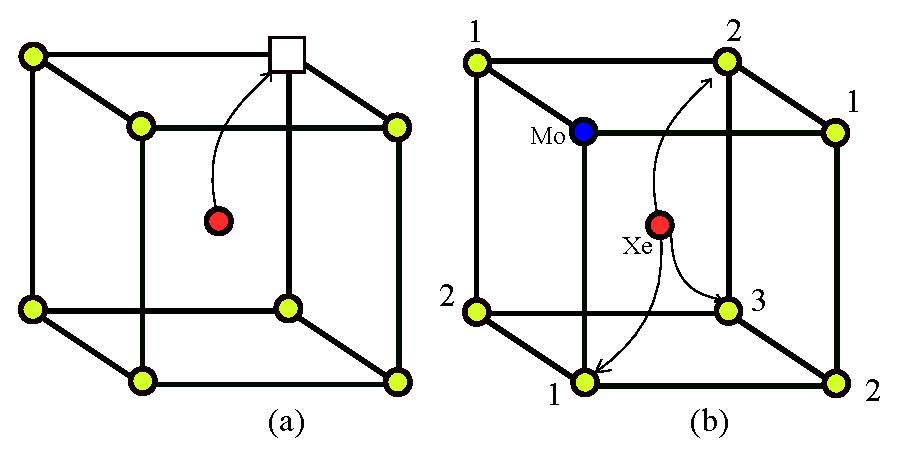
\includegraphics[scale=0.6]{image01}
	\caption[Diagram of a xenon jump from the center site to a
    nearest-neighbor vacancy in \textgamma-uranium.
    ]{Diagram of a xenon jump from the center site to a
    nearest-neighbor vacancy in \textgamma-uranium.
    (a)~All eight jumps are symmetrically equivalent with no molybdenum
    present;
    (b)~with one molybdenum atom in the nearest-neighbor shell, there are
        three unique solute jumps (1, 2, and~3).}
      \label{figure01}
\end{figure}

\begin{figure}
    \centering
    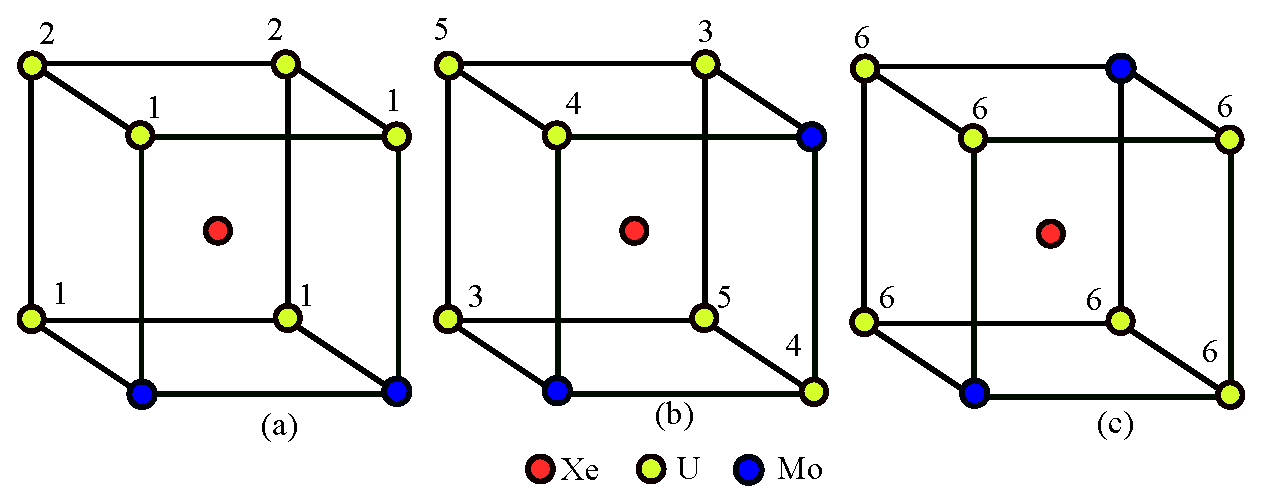
\includegraphics[scale=0.6]{2mo-1xe}
    \caption[The three sets of symmetrically-inequivalent hops of xenon from the center
        with two molybdenum atoms in the nearest-neighbor shell.]{The three sets of symmetrically-inequivalent hops of xenon from the center
        with two molybdenum atoms in the nearest-neighbor shell.
        The numbers denote symmetrically distinct pathways.}
    \label{figure02}
\end{figure}

\begin{figure}
    \centering
    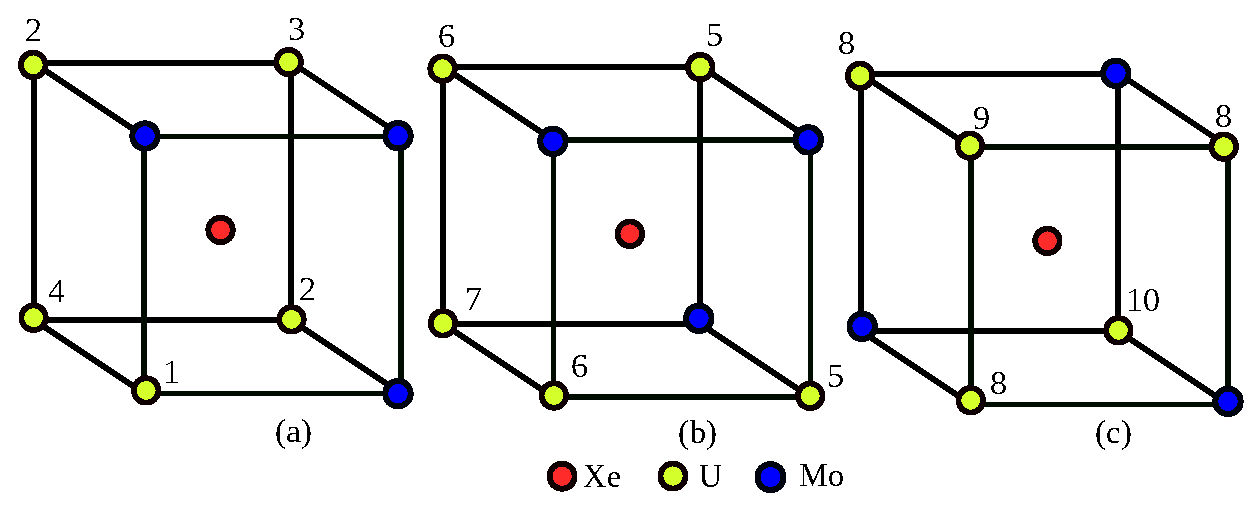
\includegraphics[scale=0.6]{3mo-1xe}
    \caption[The three sets of symmetrically-distinct hops from the center site
        with three molybdenum atoms in the nearest-neighbor shell]{The three sets of symmetrically-distinct hops from the center site with three molybdenum atoms in the nearest-neighbor shell. The numbers denote symmetrically distinct pathways.}
    \label{figure03}
\end{figure}

Figure~\ref{figure03} shows the symmetrically-distinct arrangements of three
molybdenum atoms in the nearest-neighbor shell.
This local concentration creates ten distinct jumps of a xenon atom to a
nearest-neighbor vacancy (Fig.~\ref{figure03}).
The migration energies for three-molybdenum configurations vary from 0.201~eV
for direction~5 to 1.213~eV for direction~8.
The highest migration energy is for a xenon atom that jumps to a site between
two molybdenum atoms~(site~8\ in Fig.~\ref{figure03}c).
Figure~\ref{figure03}a shows the arrangements of three molybdenum atoms on the
same \hkl(100) plane, which produces four distinct jumps with migration
energies ranging from 0.515~eV to 0.917~eV, the highest one being for
direction~2, where xenon moves to the opposite corner from the three molybdenum
atoms.
Figure~\ref{figure03}b has a combination of two molybdenum atoms on one face
of the cell and one molybdenum atom in the lower corner on the opposite site. 
This configuration reduces the migration energy compared to the configuration
in which all three molybdenum atoms are co-planar. Direction~8 (Figure~\ref{figure03}c) produces the highest migration energy for xenon. 
In this configuration, the initial minimum energy position for xenon is
equidistant from all three molybdenum atoms. The final position is not
equidistant but creates a larger activation energy. In the cases of
directions~9 and 10, the location of the vacancy changes the lowest-energy
location (final position) for xenon and reduces the barrier.
 

We did not calculate the migration energy of xenon with more than three
molybdenum atoms in the nearest-neighbor shell.
The assumption of a random (binomial)
distribution~(Table~\ref{tab_combination}) implies that the
probability of having 0--3 molybdenum atoms near a xenon solute is much higher
($>$\:96\%) than having more than three molybdenum atoms for either
U-10Mo or U-7Mo.

\section{Conclusions}
We calculated solute--vacancy binding energies for different solutes in bcc
uranium. Uranium shows relatively high vacancy--solute binding energies compared to iron and aluminum. The unstable nature of \textgamma-uranium at low temperature contributes to a significant increase in solute--vacancy binding energy relative to other bcc metals. The higher elastic binding energy in bcc uranium produces a high solute--vacancy binding energy.

We also calculated migration energies of xenon and molybdenum in pure bcc
uranium. Molybdenum's migration energy is very high compared to that of xenon,
indicating that in pure bcc uranium, xenon moves much faster than molybdenum.
The relatively low diffusivity of molybdenum also supports our assumption that
molybdenum is randomly distributed in uranium--molybdenum alloys
(presuming that the manufacturing process initially starts with a melt or
powder that produces an ideal mixture).
We also studied migration energies of xenon in the presence of molybdenum in
\mbox{U--Mo} alloys.
Different arrangements of molybdenum atoms in the nearest-neighbor shell and
xenon's distinct jumps are identified and their activation energies calculated.
The binomial distribution suggests that having up to three molybdenum atoms in
the nearest-neighbor shell is highly probable in U-10Mo and U-7Mo alloys.
The presence of molybdenum in the nearest-neighbor shell of a xenon atom has
an impact on the migration energy, but it does not generally increase or
decrease the migration energy; both the locations of the molybdenum atoms and
the direction of the jump influence the migration energy.
Having one molybdenum atom in the nearest-neighbor shell increases the
activation energy between 0.01~eV and 0.15~eV, depending on the location of
the molybdenum atom relative to the xenon atom and the vacancy.
If xenon has two molybdenum atoms nearby, we found a similar increase,
though there are combinations for which the migration energy is lower than it
is in the single-molybdenum cases.
For xenon with three nearby molybdenum atoms,
the migration energy increases for all molybdenum/\allowbreak{}vacancy
arrangements.
While there are several molybdenum arrangements that result in decreased
migration energies relative to some of the two-molybdenum configurations,
the general trend with the addition of molybdenum in the nearest-neighbor
shell near xenon is to increase the migration energy, hence reducing xenon
mobility in \mbox{U--Mo} alloys.
 
We did not consider the influence of molybdenum in the second-nearest neighbor
shell in bcc uranium. Future work should include a determination of the
effective diffusion coefficient of xenon in U--Mo alloys using the
kinetic Monte Carlo method.






\bibliographystyle{apsrev4-2}
\bibliography{abbreviated,final}
